\documentclass[12pt]{article}
\usepackage{amssymb, amsmath}
\usepackage{bm}
\usepackage{dsfont}
\usepackage{empheq}
\usepackage{graphicx}
\usepackage{float}

% Set up the margins.
\usepackage[top=1in, bottom=1in, left=1in, right=1in]{geometry}

\begin{document}



\title{DoorDash Data Science Take-Home-Assignment Report}

\author{William Wong}
\date{March 25, 2018}

\maketitle









\section{Part I. Model Building}

The work was done in a Jupyter notebook called \texttt{explore\_and\_build\_model.ipynb},
which is submitted for evaluation.

\subsection{Exploratory Analysis}


\subsection{Creating Additional Features}
We create three additional features:
\begin{enumerate}
  \item \texttt{created\_at\_hour} We extract the hour where the order is created.  This is a categorical variable.

  One can see that most orders are placed late at night (from midnight to 4 AM) and during dinner time (from 7 PM to 9 PM).
    \begin{verbatim}
    > df_csv['created_at'].dt.hour.value_counts().sort_index()

    0     12669
    1     28190
    2     36976
    3     27068
    4     15250
    5      7096
    6      1416
    7        11
    8         2
    14       40
    15      538
    16     2109
    17     3413
    18     5100
    19    13541
    20    15560
    21    11465
    22     8821
    23     8163
    Name: created_at, dtype: int64
    \end{verbatim}

  \item \texttt{created\_at\_dayofweek} We extract the hour where the day of the week is created.  This is a categorical variable.

  \item \texttt{fractional\_busy\_dashers} We define this continuous variable to be \texttt{total\_busy\_dashers} divided by \texttt{total\_onshift\_dashers}. This variable should provide some insight as to how ``loaded'' the system is.

  One can see that the system is quite busy, as the median value of \texttt{fractional\_busy\_dashers} is 0.95.

    \begin{verbatim}
    > df_csv['created_at'].dt.dayofweek.value_counts().sort_index()

    count    197421.000000
    mean          0.954620
    std           0.416678
    min           0.000000
    25%           0.846847
    50%           0.946429
    75%           1.000000
    max          34.000000
    Name: fractional_busy_dashers, dtype: float64
    \end{verbatim}

\end{enumerate}


\subsection{Summary of Features used in the Model}
% categorical
% continuous
The categorical features are:
\begin{itemize}
  \item \texttt{created\_at\_hour}
  \item \texttt{created\_at\_dayofweek}
  \item \texttt{market\_id}
  \item \texttt{order\_protocol}
\end{itemize}


The continuous features are:
\begin{itemize}
  \item \texttt{total\_items}
  \item \texttt{subtotal}
  \item \texttt{num\_distinct\_items}
  \item \texttt{min\_item\_price}
  \item \texttt{max\_item\_price}
  \item \texttt{total\_onshift\_dashers}
  \item \texttt{total\_busy\_dashers}
  \item \texttt{fractional\_busy\_dashers}
  \item \texttt{total\_outstanding\_orders}
  \item \texttt{estimated\_order\_place\_duration}
  \item \texttt{estimated\_store\_to\_consumer\_driving\_duration}
\end{itemize}


\subsection{Removing Outliers}
% Include the outcome variables.

We remove the outliers in the features and in the outcome variable and replace the values with NaN, which will be dealt with in the next stage. We consider a data point to be an outlier if the value is outside the 99-percentile of the population. An example is shown below, where the 99-percentile value of the outcome variable (\texttt{outcome\_total\_delivery\_time}) is 6475 seconds. However, there are outcome values that far exceed this number (e.g., \texttt{outcome\_total\_delivery\_time} = 8.52 million seconds!).


\begin{verbatim}
    > df_csv[col_outcome].describe(percentiles=
                                   [0.01, 0.1, 0.25, 0.5, 0.75, 0.90, 0.95, 0.99])

    count    1.974210e+05
    mean     2.908257e+03
    std      1.922961e+04
    min      1.010000e+02
    1%       1.152000e+03
    10%      1.699000e+03
    25%      2.104000e+03
    50%      2.660000e+03
    75%      3.381000e+03
    90%      4.235000e+03
    95%      4.872000e+03
    99%      6.474800e+03
    max      8.516859e+06
    Name: outcome_total_delivery_time, dtype: float64
\end{verbatim}

As an second example (Fig.~\ref{fig:total_onshift_dashers}), note that some of the values of \texttt{total\_onshift\_dashers} are negative, which are wrong.

\begin{figure}[H]
\centering
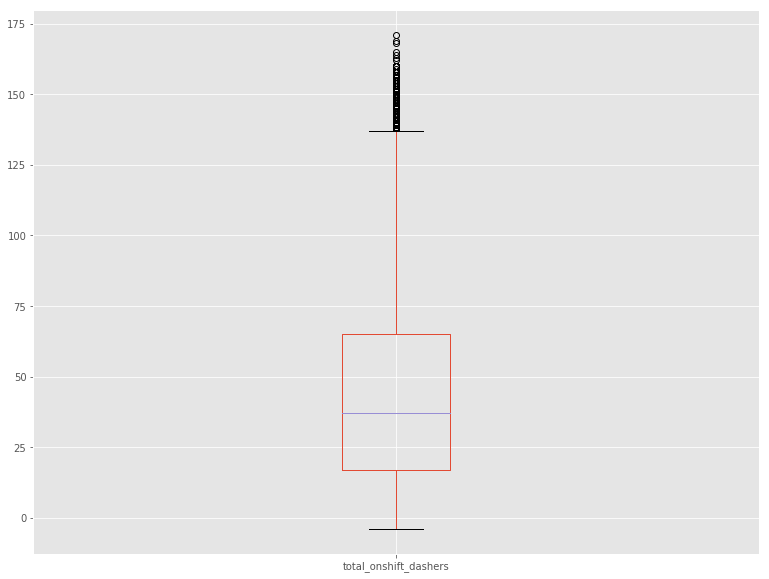
\includegraphics[width=6in]{graphics/total_onshift_dashers.png}
\caption{Box plot of the feature \texttt{total\_onshift\_dashers}.}
\label{fig:total_onshift_dashers}
\end{figure}

\subsection{Imputating Missing/Null Values}

We replace missing categorical values with the mode, and missing continuous values with the median.

We remember these operations and will repeat them during the production run.

\subsection{Training and Testing the Model}
% mention rf
To get the best performance, we model the outcome variable using random-forest regression with 200 trees.
We plot the observed outcome variable versus the predicted outcome variable, and the residual versus the predicted outcome variable in Fig.~\ref{fig:results01}.  The root-mean-squared error (RMSE) is found to be $900~\text{seconds} \pm 5\%$, which is decent (about 15 minutes).


% 2 plots of results
\begin{figure}[H]
\centering
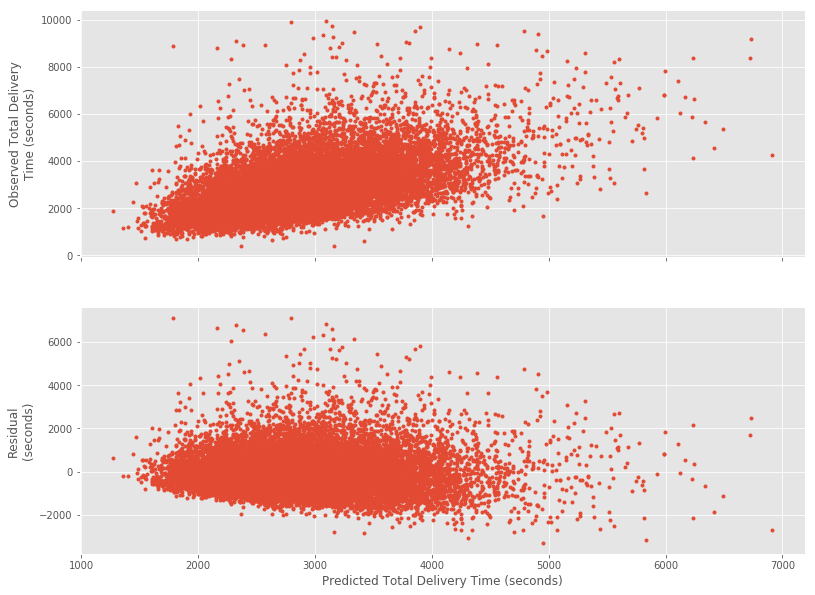
\includegraphics[width=6in]{graphics/results.png}
\caption{Plot of the observed outcome variable versus the predicted outcome variable, and plot of the residual versus the predicted outcome variable.}
\label{fig:results01}
\end{figure}






\section{Part II. The Production Run}

\subsection{The Code Base}
% unit testing
% $ python xx.py

% logging


\subsection{Cleaning of Model Features}


\subsection{Prediction of the Holdout Data Set}


\end{document}

